\chapter{Experimental Results}\label{ch:results}

\begin{flushright}
	\emph{\lq\lq A victory is twice itself when the achiever brings home full numbers.\rq\rq \\
		       \emph{Much ado about nothing}, Leonato, scene 1.}
\end{flushright}

\vspace{0.6cm}

In {\bf chapter \ref{ch:introduction}} the concept of log-composition is introduced, emphasizing its implications in medical imaging as a tool utilized in diffeomorphic registration and in the computation of the logarithm in the log-Euclidean framework. 
{\bf Chapter \ref{ch:tools}} is devoted to the introduction of the underpinning mathematical theory: it defines formally the log-composition and presents three numerical methods for its computation:
\begin{enumerate}
	\item Truncated BCH formula of degree $k=1, \frac{3}{2}, 2, 3$ - \emph{equation \ref{eq:bch_definition}}.
	\item Taylor expansion - \emph{equation \ref{eq:taylor}}.
	\item Parallel transport - \emph{equation \ref{eq:parallel_transport}}.
\end{enumerate}
Before evaluating their results on the SVF, some tests in the are is evaluated for two groups of transformation, {\bf chapter \ref{ch:spatial_transformations}} introduces two groups of transformations:
\begin{enumerate}
	\item The finite dimensional Lie group of euclidean transformation SE(2), where a closed form of the log-composition is known - \emph{section \ref{se:rigid_body_transformations}}
	\item The infinite dimensional Lie group diffeomorphisms, set of images of SVF through the Lie exponential map - \emph{section \ref{se:svf}}
\end{enumerate}
For each of these groups it presents as well the numerical methods for the computation log-composition shown in the previous chapter for the general case.
{\bf Chapter \ref{ch:log_algorithm}} is about the algorithm for the computation of the Lie logarithm \cite{Bossa:08}, called here log-algorithm. 
Thanks to the fact that this important piece in the jigsaw puzzle of the log-euclidean framework can be reformulated in term of the log-composition, it is possible to compute it using numerical methods introduced:
\begin{enumerate}
	\item Truncated BCH formula of degree $k=1, \frac{3}{2}, 2, 3$ - \emph{equation \ref{eq:bossa_bch_strat}}.
	\item Parallel transport - \emph{equation \ref{eq:bossa_parallel_strategy}}.
	\item Symmetric parallel transport - \emph{equation \ref{eq:bossa_symmetric}}.
\end{enumerate}

This last chapter is devoted to show some of the results of the numerical methods investigated.
Computations are performed with a software written in Python (repository available on the \href{https://cmiclab.cs.ucl.ac.uk}{cmic gitlab}), based on 
the following libraries - numpy, matplotlib, math, scipy, nibabel, timeit, random - as well as on the library NiftyBit, implemented by Pancaj Daga.

% % % % % % % % % % % % % % % % % % % % % % % % % % % % % % % % % % % % % %
% % % % % % % % % % % % % % % % % % % % % % % % % % % % % % % % % % % % % % 
% % % % % % % % % % % % % % % % % % % % % % % % % % % % % % % % % % % % % % 
\section{Log-composition for $\mathfrak{se}(2)$}

There are several norms in the space of $3\times 3$ squared matrices that can be inherited by the group $SE(2)$ and the Lie algebra $\mathfrak{se}(2)$ when represented by matrices. For our tests we considered the tangent space $\mathfrak{se}(2)$ with the inherited Frobenius norm:
\begin{align*}
\euclideanMetric{(\theta,dt^{x},dt^{y})}_{\text{fro}} = \sqrt{2\theta^{2} + (dt^{x})^2 + (dt^{y})^2} 
\qquad
(\theta,dt^{x},dt^{y}) \in \mathfrak{se}(2)
\end{align*}
Numerical tests show that for the studied cases, no qualitative differences are detected if choosing instead the $L^{2}$ norm.
 %
 \begin{figure}[!ht]
 	\hspace{-2cm}
 	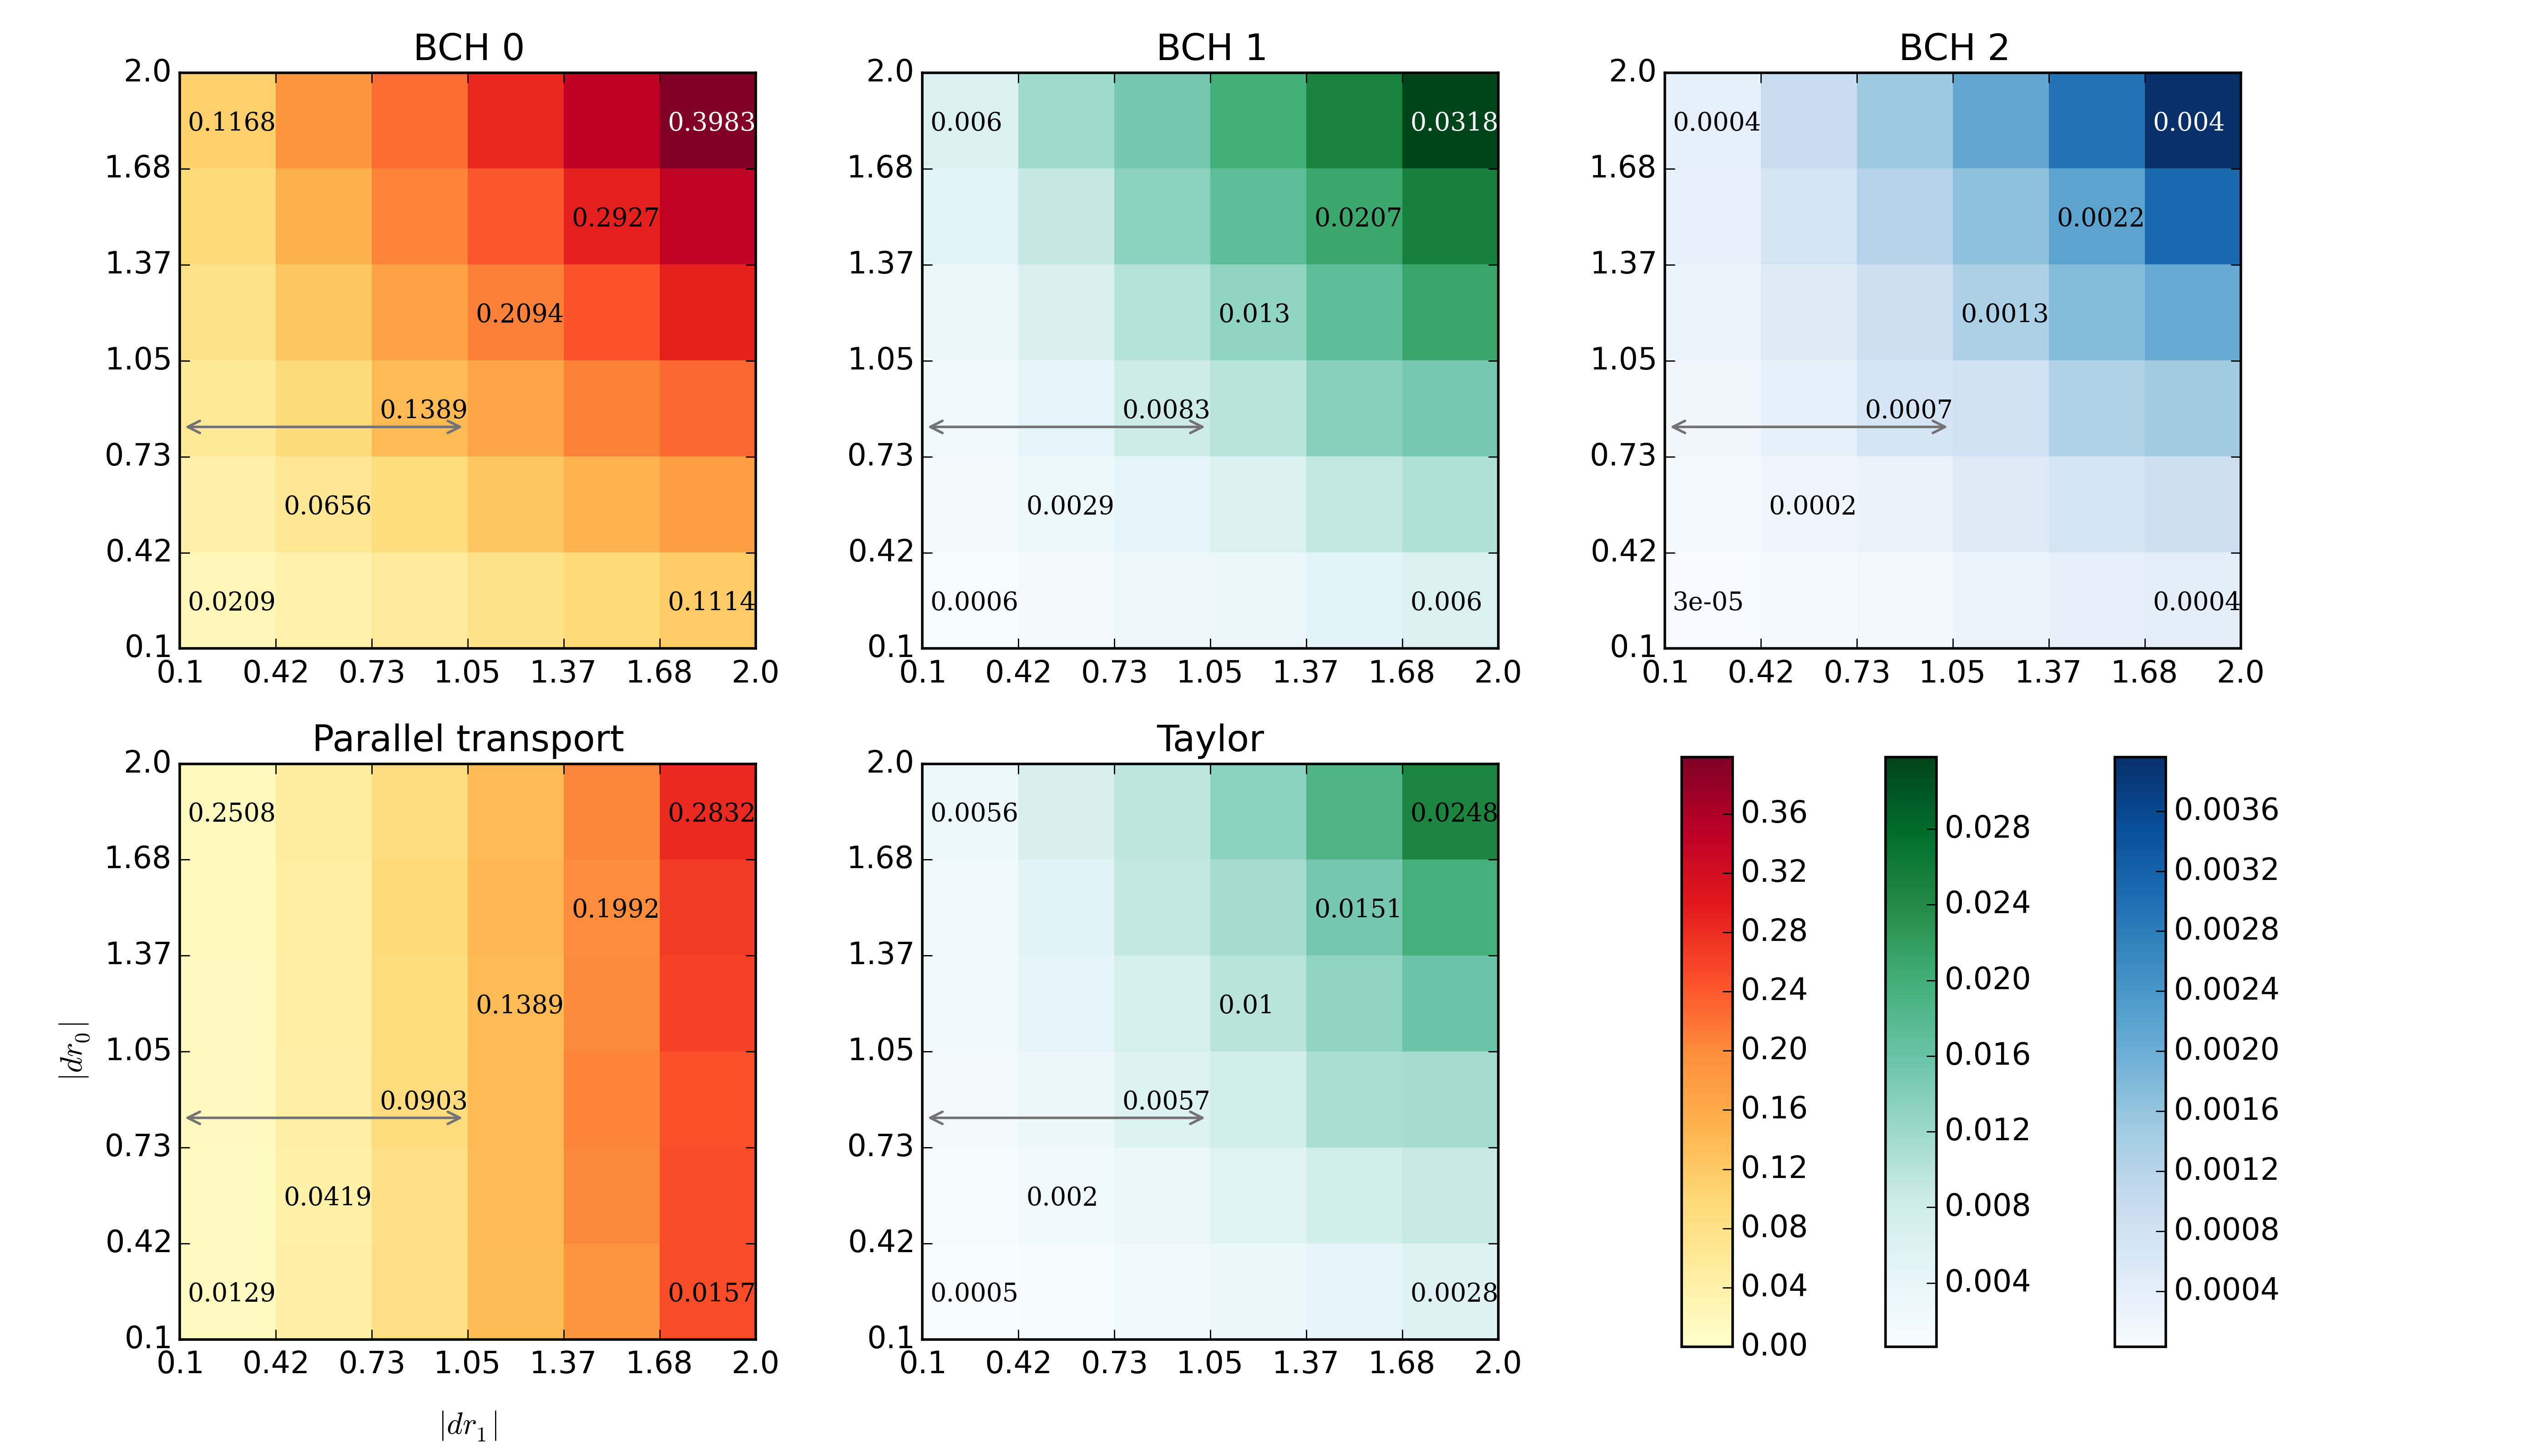
\includegraphics[scale=0.54]{figures/se2_image_scale.png}
 	\caption{Comparison of the errors for each numerical method to compute the Log-composition $dr_{0} \oplus dr_{1}$ in $\mathfrak{se}(2)$. Truncated BCH of degrees 0,1,2, parallel transport method and Taylor method are considered for different values of the norm of $dr_{1}$ (x-axes) and norm of $dr_{0}$ (x-axes). 
 	Values of each sub-square are the average error of 500 random samples in each of the 6 sub-intervals between $0.1$ and $2.0$. Errors with BCH 0 and parallel transport method are comparable, but the parallel transport method is not symmetric and has better performance when $dr_{1}$ is small. BCH 1 and Taylor are comparable as well, but the best performance in terms of approximation is the BCH 2. Values of the sub-square under the \emph{gray arrows} are shown in the boxplot \ref{fig:se2_image_scale} where variance, quartiles and outliers are visualized.
 	 }
 	\label{fig:se2_image_scale}
 \end{figure}
 %
% % % % % % % % % % % % % % % % % % % % % % % % % % % % % % % % % % % % % %
% % % % % % % % % % % % % % % % % % % % % % % % % % % % % % % % % % % % % % 
\subsection{Methods and Results}

To compare the errors the computation of the log-composition for the methods presented, two sets of $3000$ transformations of elements in $\mathfrak{se}(2)$ are randomly sampled with increasing norms in the interval $[0.1, 2.0]$. This interval is divided into 6 segments delimited by $ I = \text{linspace}([0.1, 2.0], 7)$ and for each couple of subintervals $[I(n_0), I(n_0+1)]$, $[I(n_1), I(n_1+1)]$ two sets of $500$ transformations $\{ dr_{0}^{(j)}\}_{j=1}^{500}$, $\{ dr_{1}^{(j)} \}_{j=1}^{500}$ having norms belonging to the respective intervals are sampled:
\begin{align*}
j=1,...,500 \quad &\quad  n_0, n_1 = 0,...,5 \\
\euclideanMetric{dr_{0}^{(j)}}_{\text{fro}} &\in [I(n_0), I(n_0+1)] \\
\euclideanMetric{dr_{1}^{(j)}}_{\text{fro}} &\in [I(n_1), I(n_1+1)]  
\end{align*} 
If $N$ is one of the numerical methods presented in section \ref{se:rigid_body_transformations} for the computation of the log-composition - $\text{BCH}^{0}, \text{BCH}^{1}, \text{BCH}^{2}, \text{Tl}, \text{pt}$ - 
then the error between the ground truth and the approximation provided by one of these numerical methods is given by
\begin{align*}
\text{Error}(dr_{0},dr_{1},N) 
:= 
\euclideanMetric{dr_{0}^{(j_0)} \oplus dr_{1}^{(j_1)} 
- 
N(dr_{0}, dr_{1}) }_{\text{fro}} 
\end{align*}

In figure \ref{fig:se2_image_scale}, each of the figure corresponds to a different method and each of the grade scale is the value computed with the function:
\begin{align*}
f(n_0,n_1,N) 
=
 \mathbb{E}\Big(
  \{ 
  \text{Error}(dr_{0}^{(j)},dr_{1}^{(j)},N) 
  \}_{j=1}^{500}
  \Big)
\end{align*}
Where the norm of $dr_{0}^{(j)}$ belongs to the interval $[I(n_0), I(n_0+1)]$ and the norm of 
$dr_{1}^{(j)}$ belongs to $[I(n_1), I(n_1+1)]$, and where $\mathbb{E}$ is the mean value.\\
The data indicated by the gray arrows in each plot corresponds are showed in the box-plot \ref{fig:se2_boxplot}
%
\begin{figure}[!ht]
	\hspace{-1.5cm}
	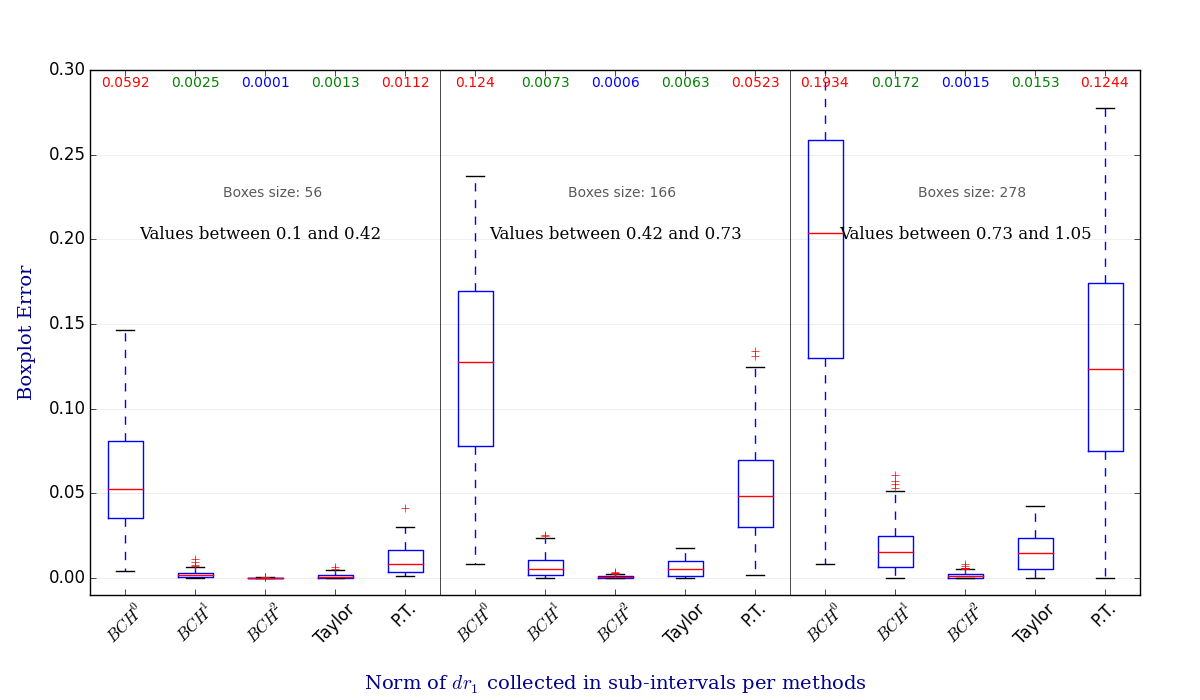
\includegraphics[scale=0.54]{figures/se2_boxplot.png}
	\caption{Errors of the numerical methods for the computation of the Log-composition of $dr_{0} \oplus dr_{1}$ in $\mathfrak{se}(2)$. Norm of $dr_{0}$ is in the interval $[0.37,1.05]$, norm of $dr_{1}$ in the interval $[0.1, 1.05]$ divided in 3 segments. Mean values of each box are shown in the first row in different colors. Shown data corresponds to a section of the image scale \ref{fig:se2_image_scale}, indicated by a gray arrow. As expected all of the error means increase with the of norm of $dr_1$, but the rate of the growth is different for each method.}
	\label{fig:se2_boxplot}
\end{figure}
%

From these results in $\mathfrak{se}(2)$ we can see that the second truncation error of the BCH formula provides the best result (the unit of measure is the same as the measure chosen for the translation or the rotation: it can be inches, cm, pixel, ...).

Method based on the $BCH^0$, that is utilized for example in the additive demons, do not involves any Lie bracket. Its results show that the bigger is the norm of the transformation involved, the bigger is its Lie bracket and its nested Lie bracket as appears in the $BCH^1$ and $BCH^2$. Do not take into account Lie brackets means do not take into account the curvature of the space \cite{misner1973gravitation}, whose significance is given by the experimental results. Parallel transport method tries to compensate the curvature using a geometrical approach considering different tangent spaces to the manifold of the transformation than the one at the origin. As expected from the formula is not symmetric. It provides better results than the $BCH^0$, and when the norm of $dr_1$ is small, results are close to the one obtained with $BCH^1$ when norms of $dr_0$ and $dr_1$ are below $1.3$.

Log-composition based on Taylor method has slightly better results than the $BCH^1$, but do not reach $BCH^2$, which provides the best results. This may be due to the fact that the Taylor belongs to $\mathcal{O}(dr_1^2)$ while the $BCH^2$ involves the Lie bracket $[dr_0,[dr_0, dr_1]] + [dr_1,[dr_1, dr_0]]$. Even if the truncated $BCH$ does not have a known asymptotic error (or big-O notation), this last observation provides that $BCH^2$ have a bigger asymptotic order of converges than $\mathcal{O}(dr_1^2)$, in $\mathfrak{se}(2)$.


% % % % % % % % % % % % % % % % % % % % % % % % % % % % % % % % % % % % % %
% % % % % % % % % % % % % % % % % % % % % % % % % % % % % % % % % % % % % %
% % % % % % % % % % % % % % % % % % % % % % % % % % % % % % % % % % % % % % 
% % % % % % % % % % % % % % % % % % % % % % % % % % % % % % % % % % % % % % 
\section{Log-composition for SVF}
Before getting into the results for the log-composition of SVF it is important to spend some words about how random SVF are created and how to compare the norm of the approximation of $\mathbf{u}_0\oplus \mathbf{u}_1$ with the ground truth when this is not available.
%
\begin{figure}[!ht]
	\hspace{-0.8cm}
	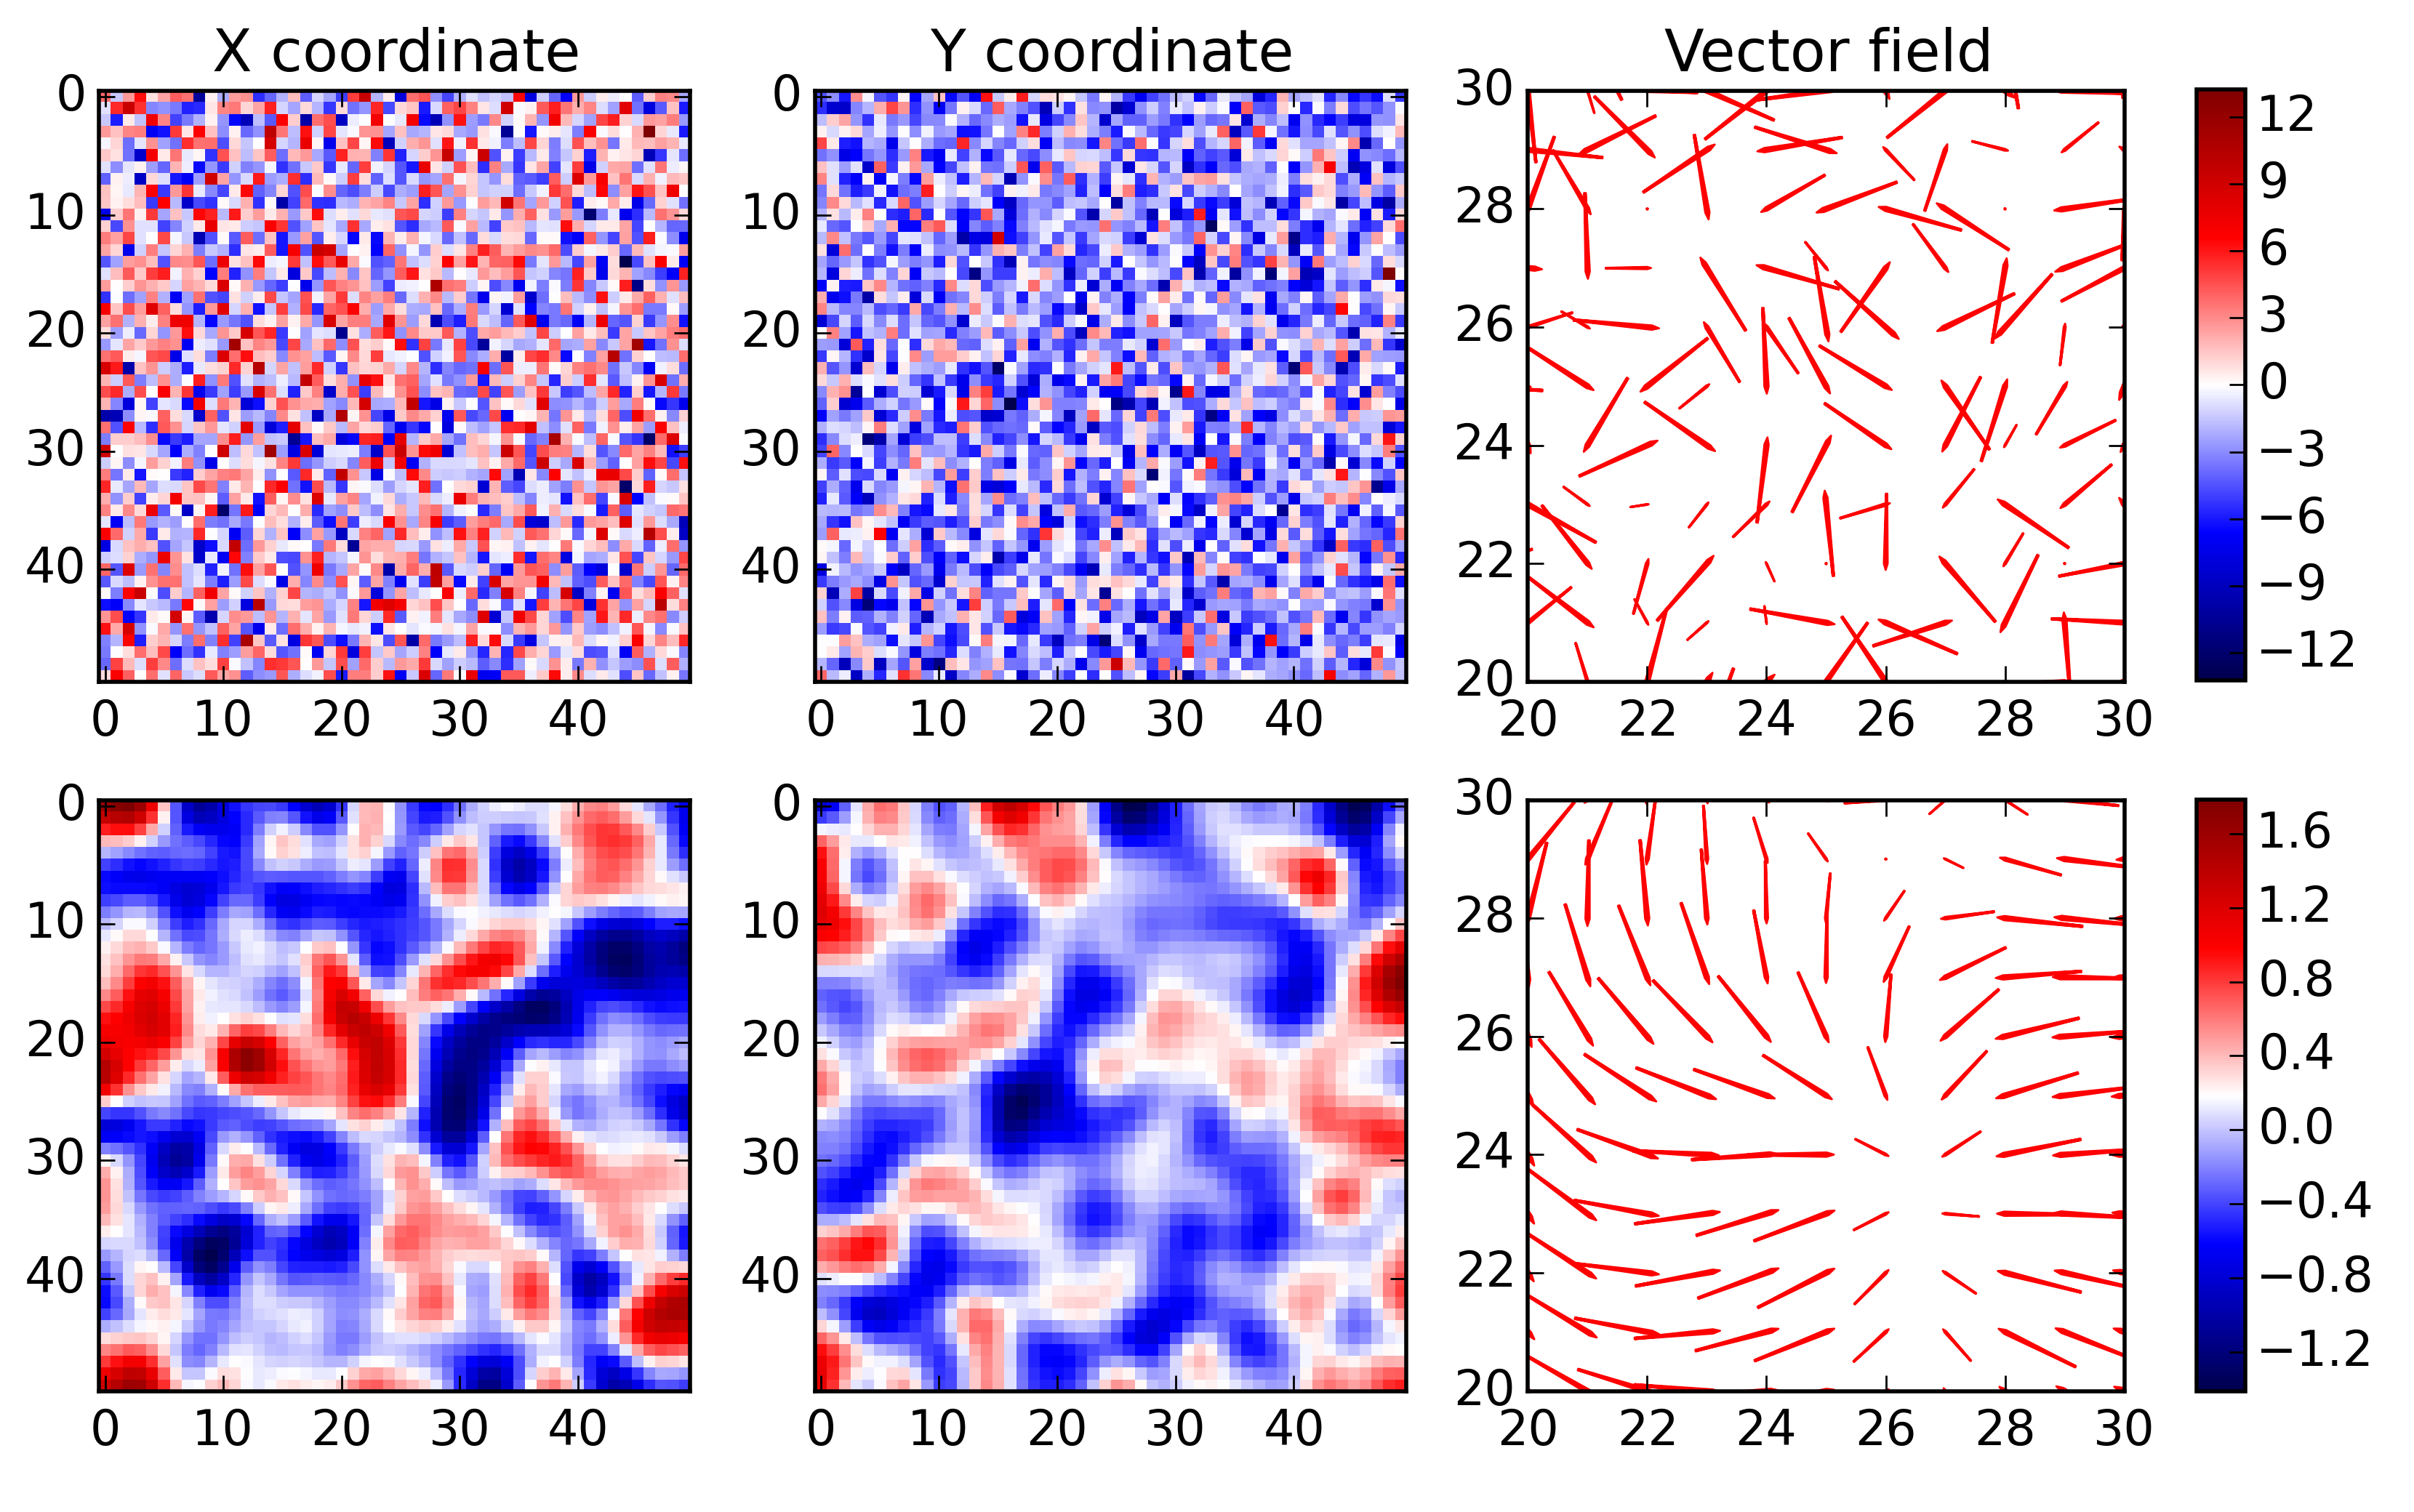
\includegraphics[scale=0.72]{figures/svf_gaussian_smoothing_effects.png}
	\caption{Random generated vector field before and after the Gaussian smoother: in the first row a random generated vector field of dimension $50\times 50 \times 2$ where the value at each pixel are sampled from a random variable with normal distribution of mean $0$ and sigma $4$. The second row shows the same random vector field after a Gaussian smoothing of sigma $2$ (the code is based on the scipy library ndimage.filters.gaussian\textunderscore filter). In the last column shows the quiver of the vector field in the squared subregion of size $10\times 10$ at the point $(20,20)$. From the colorscale it is also possible to see that the values distribution of the filtered image is not anymore symmetric. }
	\label{fig:SVF_gaussian_smoothing_effects}
\end{figure}
% % % % % % % % % % % % % % % % % % % % % % % % % % % % % % % % % % % % % %
% % % % % % % % % % % % % % % % % % % % % % % % % % % % % % % % % % % % % % 
\subsection{Methods: random generated SVF and ground truth.}

DRAFT:
\begin{itemize}
\item How to generate a random SVF - formula refer to figure \ref{fig:SVF_gaussian_smoothing_effects}
\item Norm defined in both Lie algebra and Lie group, thanks to the fact that ... inheritance. formula
\item How the norm changes with the space and with the filter: \ref{fig:SVF_sigma_means_comparisons}
\item How the norm affect the Lie bracket: 
\end{itemize}

We will exploit the parametrization of discretized SVF using matrices to have a ground truth to compare results. 

Norm will be computed in the group as the $L_2$ norm of matrices that represents the SVF. \\ 
Given $\mathbf{u}$ and $\mathbf{v}$ in $\text{\emph{Diff}}^{1}(\Omega)$, $\mathbf{w}_{\text{ground}} = \mathbf{u}\oplus \mathbf{v}$ solution of the log-composition and $\mathbf{w}_{\text{app}}$ its approximation using a numerical method, then their difference is computed in the group as:
\begin{align*}
\text{error} = \euclideanMetric{\exp(\mathbf{w}_{\text{ground}}) - \exp(\mathbf{w}_{\text{app}})}_{L^{2}}
\end{align*}
where $\exp(\mathbf{w}_{\text{ground}})$ is computed as the composition of the exponentials of $\mathbf{u}$ and $\mathbf{v}$:
\begin{align*}
\exp(\mathbf{w}_{\text{ground}}) = \exp(\mathbf{u})\circ \exp(\mathbf{v})
\end{align*}
As previously said, the norm $L^2$ is considered improperly in a group structure. It can be done only thanks to the fact that the discrete SVF and the corresponding diffeomorphisms $\text{\emph{Diff}}^{1}(\Omega)$ are implemented with 5-dimensional matrices (see equation \ref{eq:basic_data_structure}).
%(TODO: restate this in the limitations suggesting an alternative computation of the error as future work)\\




\begin{figure}[!ht]
	\hspace{-1.5cm}
	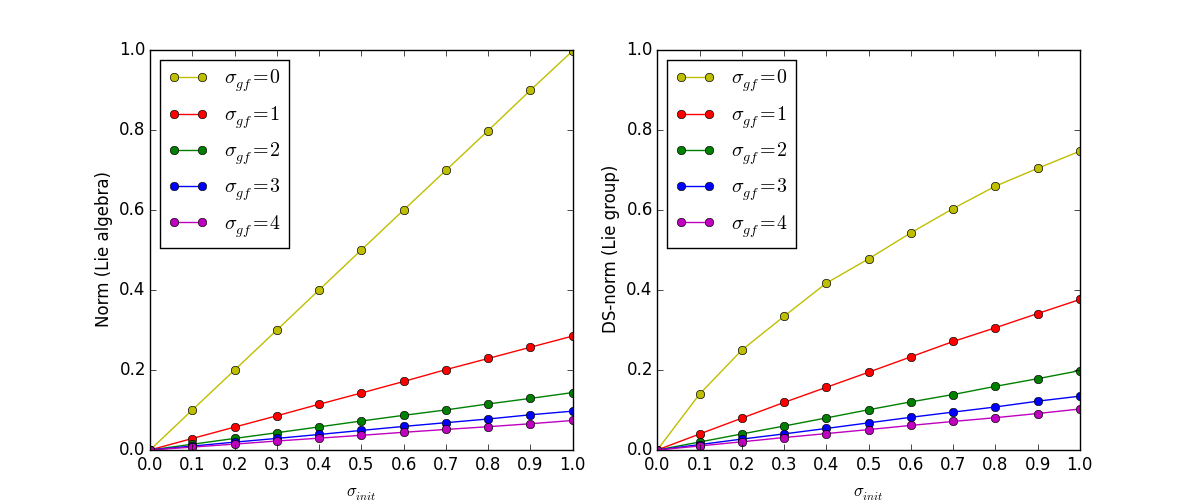
\includegraphics[scale=0.54]{figures/SVF_sigma_means_comparisons.png}
	\caption{Norm of random generated of SVF with initial standard deviation $\sigma_{\text{init}}$ (on the x-axis) and Gaussian filter with standard deviation $\sigma_{\text{gf}}$ (different colors). On the left is shown the the Frobenius norm computed on the SVF in the Lie algebra, while on the right the same norm is computed after the exponentiations. In this second case, the norm refers to the norm of the matrix data structure (DS-norm) utilized to parametrize the SVF. Each dot represents the mean of the norm of $10$ an SVF randomly generated with the parameters indicated on the axes and in the legend. We observe that the exponential bend the shape of the random SVF when the Gaussian filter is $0$ (thus we talk about an improper SVF). The decrease in the slope when $\sigma_{\text{gf}}=0$ do not appears for any other value.}
	\label{fig:SVF_sigma_means_comparisons}
\end{figure}

\begin{figure}[!ht]
	\hspace{-1cm}
	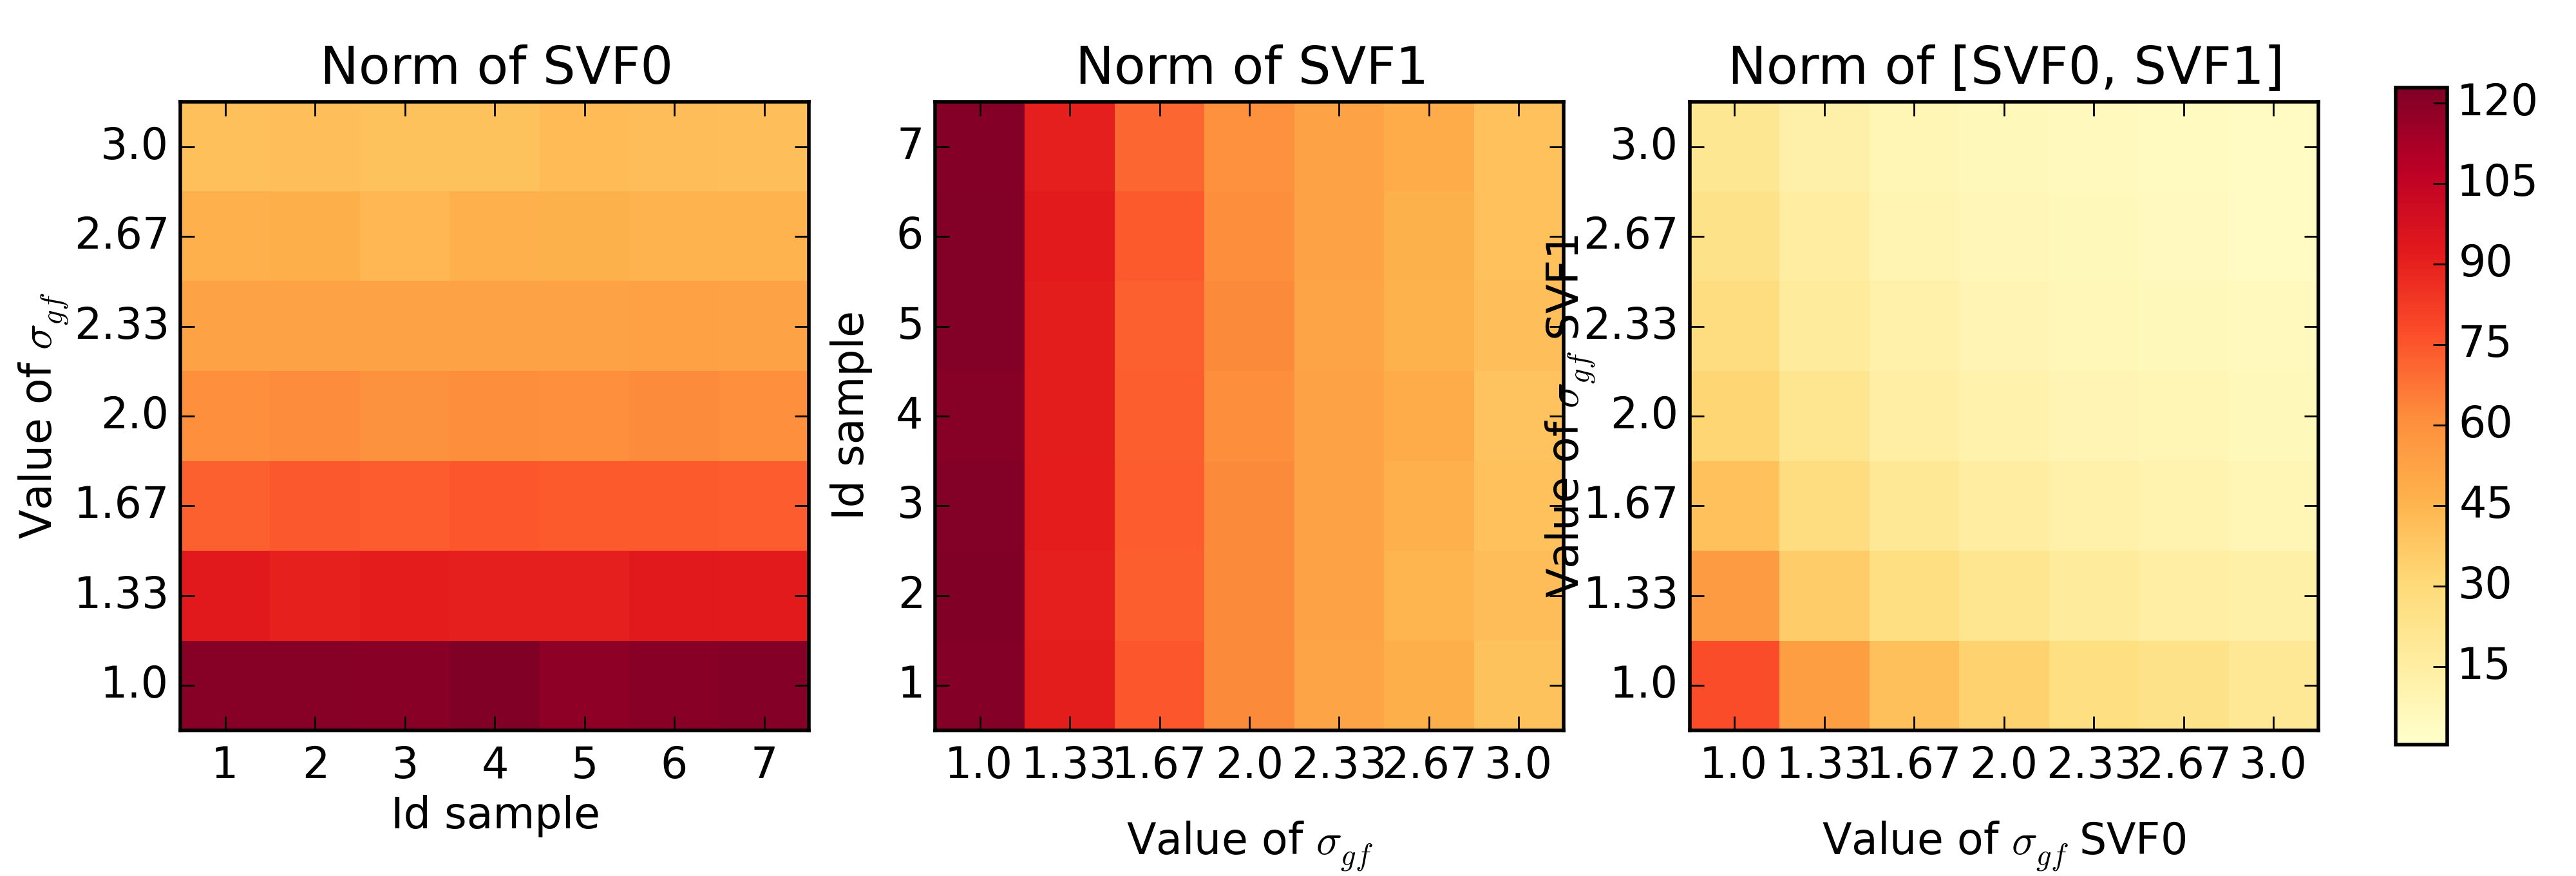
\includegraphics[scale=0.6]{figures/SVF_image_scale_bracket_versus_gaussian.png}
	\caption{Norm of the Lie bracket as direct consequence of the sigma of the Gaussian smoother of respective SVF. Here put every other data!}
	\label{fig:SVF_image_scale_bracket_versus_gaussian}
\end{figure}





\begin{figure}[!ht]
	\hspace{-1.5cm}
	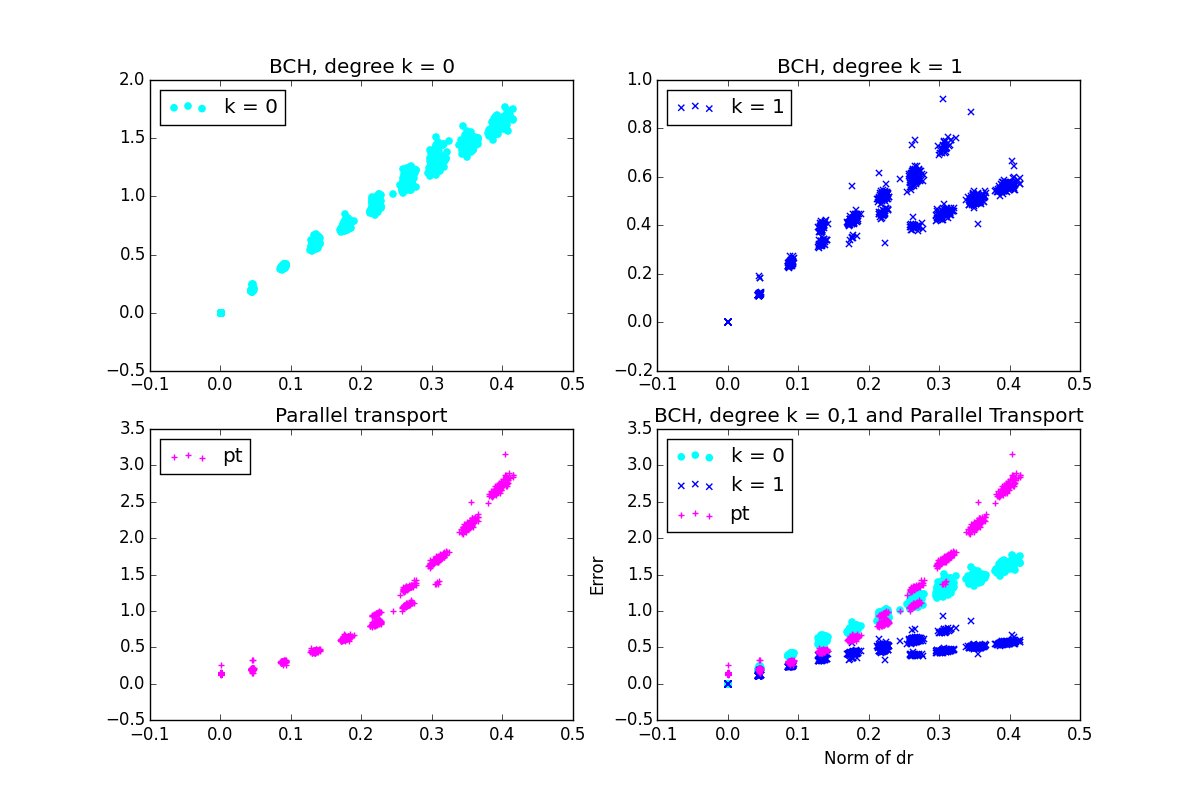
\includegraphics[scale=0.6]{figures/SVF_bch_parallel_transport.png}
	\caption{Log-composition for SVF computed using numerical methods of truncated BCH of degree 0,1 and parallel transport.}
	\label{fig:SVF_bch_parallel_transport}
\end{figure}


\begin{figure}[!ht]
	\hspace{-2.1cm}
	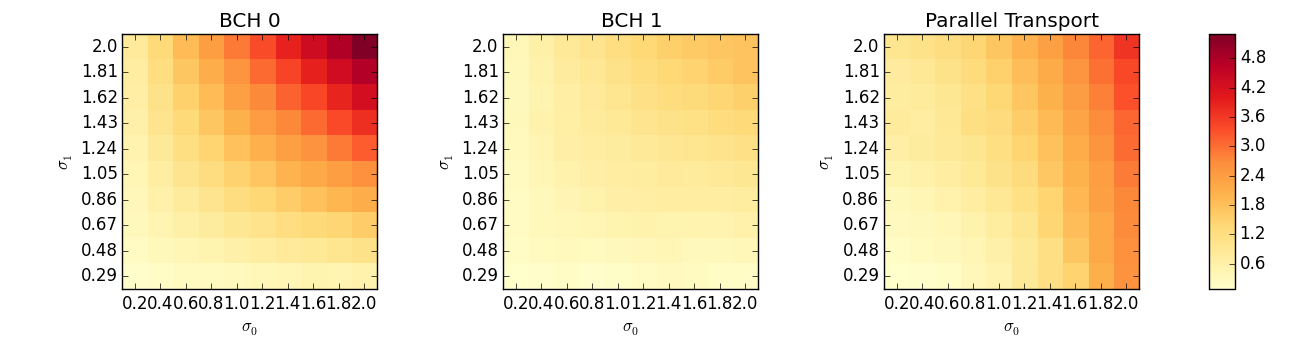
\includegraphics[scale=0.53]{figures/SVF_image_scale.png}
	\caption{Log-composition for SVF; the operation $\mathbf{u}_0\oplus \mathbf{u}_1$ is computed using numerical methods of truncated BCH of degree 0,1 and parallel transport. Respective standard deviation of the random generated SVF given by $\sigma_0$ and $\sigma_1$, ranges between $0.3$ and $2.0$ for $\sigma_0$ and between $0.2$ and $2.0$ for $\sigma_1$. Each value in the image scale is the mean of $10$ results of the log-computation of random SVF generated with given standard deviation. For lower values of $\mathbf{u}_1$, that in the image registration algorithms are given by the update, parallel transport method and truncated BCH of degree 1 have comparable results. We can also notice that for truncated BCH methods the results are symmetric, while for parallel transport, as expected from the formula, results are not symmetric respect to the size of the input vectors. }
	\label{fig:SVF_image_scale}
\end{figure}


\begin{figure}[!ht]
	\hspace{-2cm}
	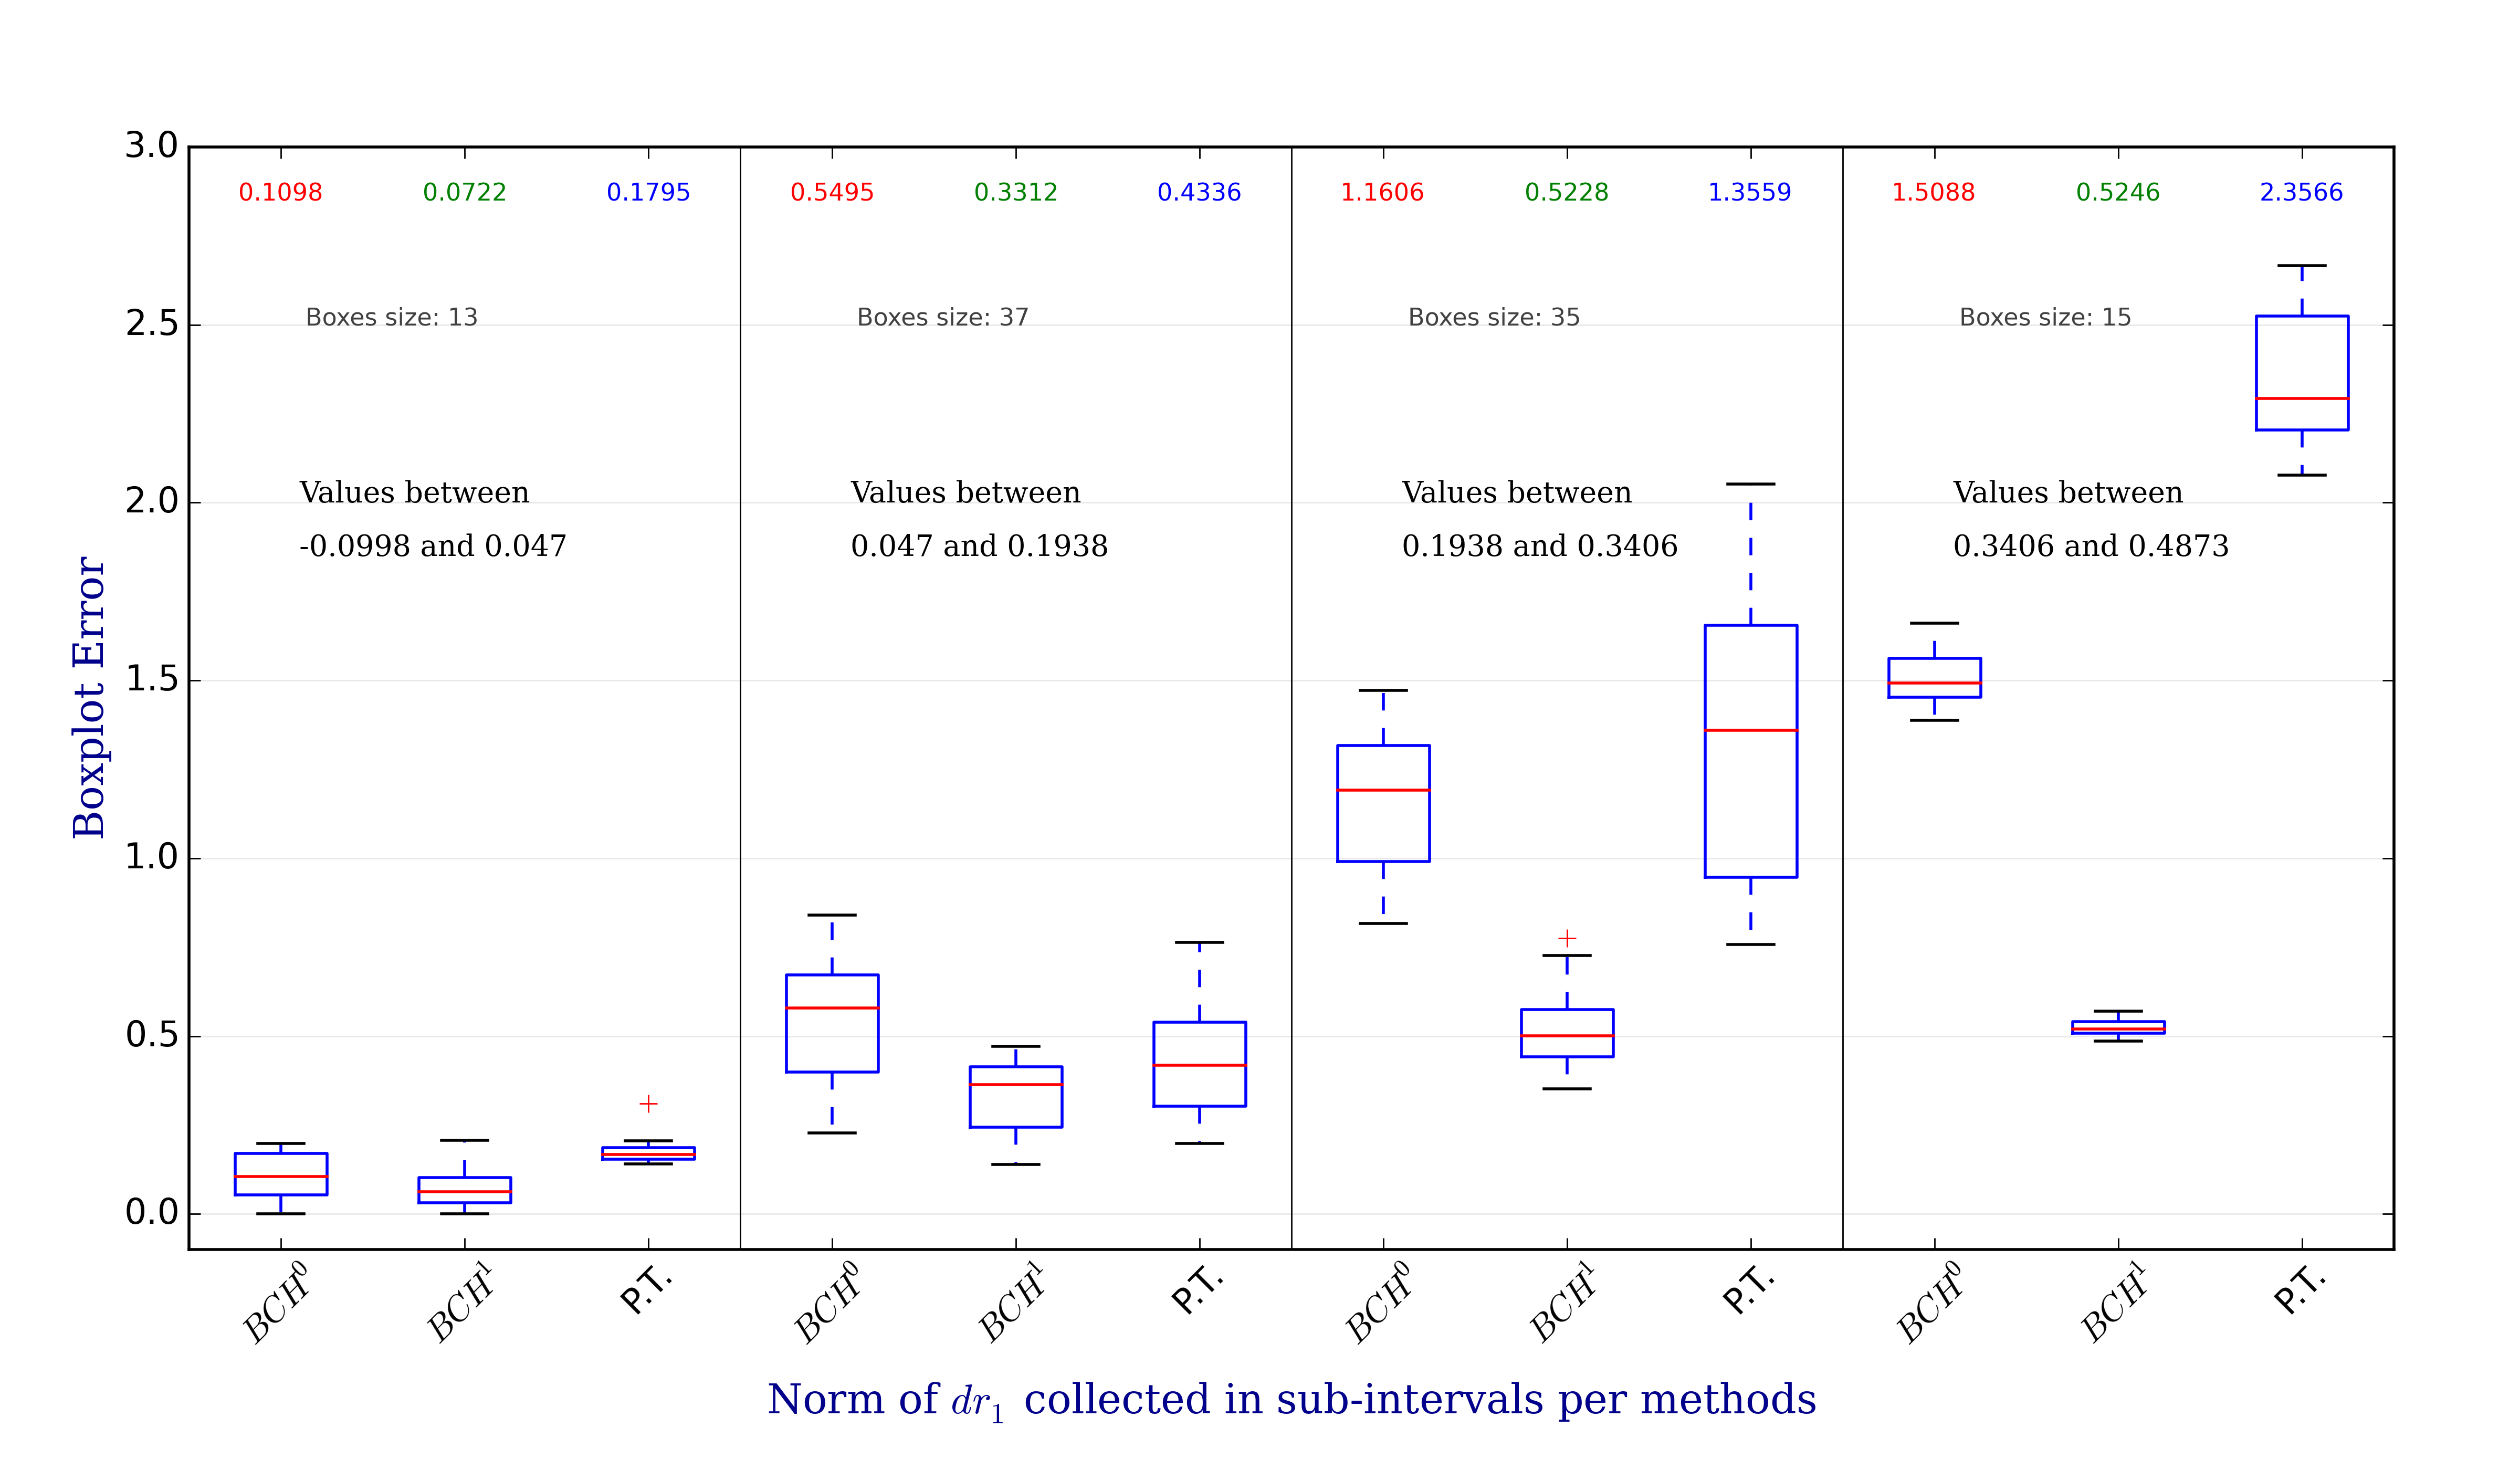
\includegraphics[scale=0.6]{figures/SVF_boxplot.png}
	\caption{Log-composition for SVF computed using numerical methods of truncated BCH of degree 0,1 and parallel transport, represented in a boxplot.}
	\label{fig:SVF_boxplot}
\end{figure}










% % % % % % % % % % % % % % % % % % % % % % % % % % % % % % % % % % % % % %
% % % % % % % % % % % % % % % % % % % % % % % % % % % % % % % % % % % % % % 
\subsection{Methods and results}


comment figures 5.6, 5.7, 5.8.

% % % % % % % % % % % % % % % % % % % % % % % % % % % % % % % % % % % % % %
% % % % % % % % % % % % % % % % % % % % % % % % % % % % % % % % % % % % % % 
\section{Log composition applied to SVF from real cases}

zzz see of you have time!

% % % % % % % % % % % % % % % % % % % % % % % % % % % % % % % % % % % % % %
% % % % % % % % % % % % % % % % % % % % % % % % % % % % % % % % % % % % % % 
% % % % % % % % % % % % % % % % % % % % % % % % % % % % % % % % % % % % % % 
\section{Log-Algorithm for SVF}

% % % % % % % % % % % % % % % % % % % % % % % % % % % % % % % % % % % % % %
% % % % % % % % % % % % % % % % % % % % % % % % % % % % % % % % % % % % % % 
\subsection{Methods}

% % % % % % % % % % % % % % % % % % % % % % % % % % % % % % % % % % % % % %
% % % % % % % % % % % % % % % % % % % % % % % % % % % % % % % % % % % % % % 
\subsection{Results}


% % % % % % % % % % % % % % % % % % % % % % % % % % % % % % % % % % % % % %
% % % % % % % % % % % % % % % % % % % % % % % % % % % % % % % % % % % % % % 
\section{Empirical Evaluations of Computational Time}


% % % % % % % % % % % % % % % % % % % % % % % % % % % % % % % % % % % % % %
% % % % % % % % % % % % % % % % % % % % % % % % % % % % % % % % % % % % % %
% % % % % % % % % % % % % % % % % % % % % % % % % % % % % % % % % % % % % % 
\section{Conclusions and Further Research}\label{ch:conclusions}


Considering only the results, this one-year research can be considered much ado about nothing, but...\\
Computational time...!

Starting from the definition of Lie log-group of diffeomorpshisms $(\mathfrak{g} , \oplus)$, to have an algebraic definition of this approximation, we can consider its quotient over the ideal generated by $(\text{ad}_{\mathbf{u}}^{m}, \text{ad}_{\mathbf{u}}^{n})$, which provides the group $(\quotient{\mathfrak{g}}{(\text{ad}_{\mathbf{u}}^{m}, \text{ad}_{\mathbf{u}}^{n})}, \oplus)$. Further investigations in this direction is not prosecuted.


The BCH is proved only when the exp and log can be expressed in power series, so when the Lie group and the Lie algebra involved belongs to the same bigger group. This is not the case of the infinite dimensional Lie group of diffeomorphisms,